\clearpage
\subsection{Image-derived feature distributions}
The histograms summarize available baseline structural MRI measurements in cubic millimetres. Each bar counts observations within a volume interval.

\begin{figure}[!ht]
\centering
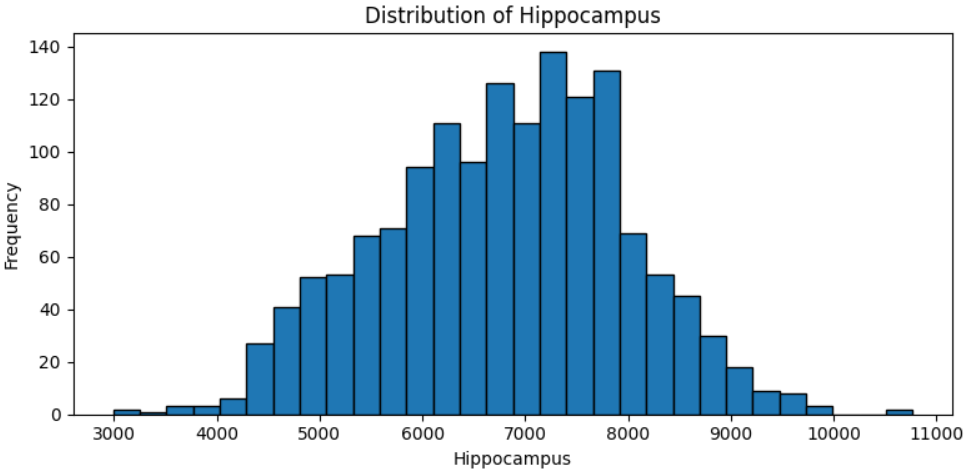
\includegraphics[width=.78\linewidth]{figures/hippocampus_distribution.png}\par\smallskip
{\small (a) Hippocampal volume.}\par\medskip
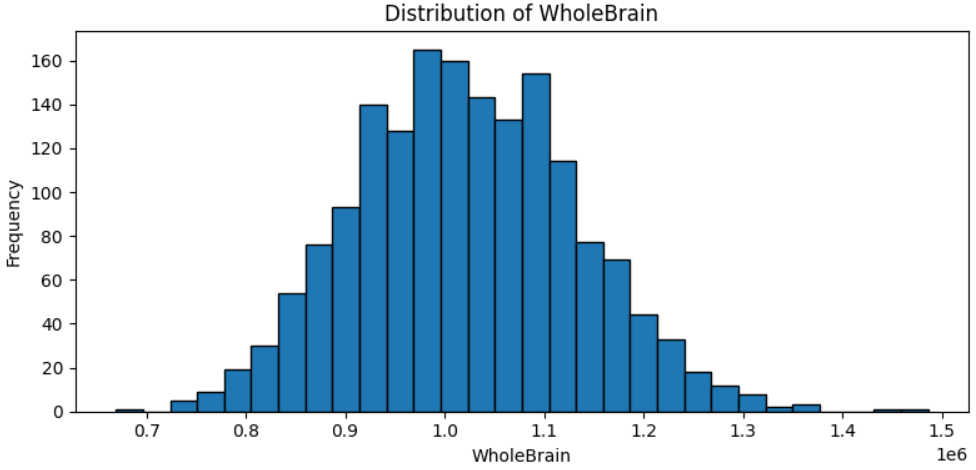
\includegraphics[width=.78\linewidth]{figures/whole_brain_distribution.png}\par\smallskip
{\small (b) Whole-brain volume.}
\caption{Distributions of observed hippocampal and whole-brain volumes.}
\label{fig:ritam-mri-distributions}
\end{figure}

Hippocampal volumes are concentrated around 7,000--7,500~mm$^3$, with a longer tail toward smaller values. Whole-brain volumes form a roughly symmetric distribution centred near $1.0\times10^6$~mm$^3$. Whole-brain volume has more recorded observations than hippocampal volume, so the two plots describe samples of different sizes. These pooled distributions show the spread of measured values. The group comparison on the next page examines how those measurements vary with baseline diagnosis.

\clearpage
\subsection{MRI volume ratios by current baseline diagnosis}
Dividing each volume by intracranial volume (ICV) expresses it as a fraction of head size. In each box plot, the centre line marks the median and the box spans the middle half of observed values. CN denotes cognitively normal participants and MCI denotes mild cognitive impairment. The sample count for each group appears below its box.

\begin{figure}[!ht]
\centering
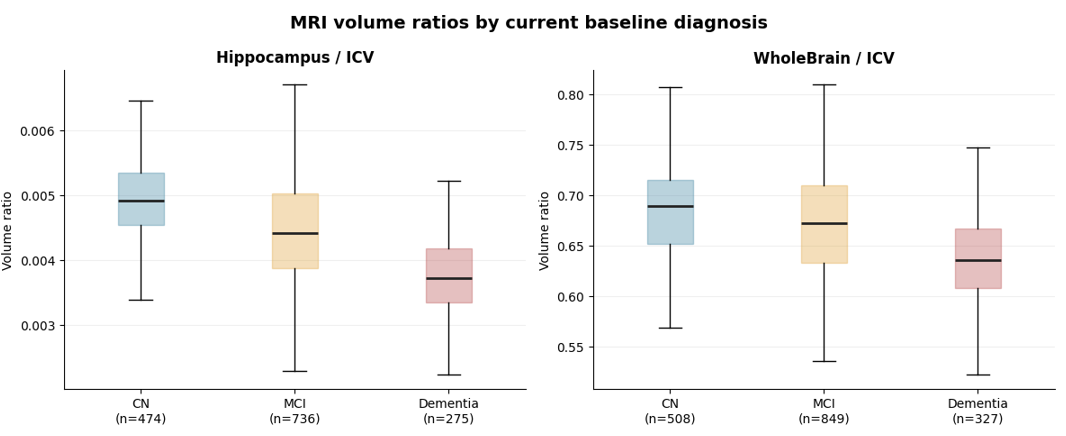
\includegraphics[width=\linewidth]{figures/mri_volume_ratios.png}
\caption{Hippocampal and whole-brain volumes relative to ICV, grouped by current baseline diagnosis.}
\label{fig:ritam-mri-ratios}
\end{figure}

For both ratios, the median is highest in CN, intermediate in MCI and lowest in dementia. The hippocampal ratio falls from approximately 0.0049 to 0.0044 to 0.0037 across the three groups. The whole-brain ratio falls from about 0.69 to 0.67 to 0.64. The boxes and whiskers overlap, so an individual's ratio alone provides limited information about their diagnosis. The sample counts differ between the two plots because each ratio requires its own volume measurement in addition to ICV.

Prior ADNI research linked MRI-measured hippocampal atrophy to subsequent progression from MCI to Alzheimer's disease \cite{jackmri}. This report's figure compares diagnoses at baseline in the exploratory cohort. It includes participants who already had dementia, whereas the five-year prediction cohort excludes them. The final predictor uses the original MRI quantities with training-fitted scaling.

\clearpage
\subsection{Supplementary cognitive features}
Everyday Cognition (ECog) measures how cognitive difficulties affect daily activities \cite{fariasecog}. The supplementary feature block includes study-partner (SP) and participant (Pt) reports, along with separate neuropsychological test scores.

{\small\renewcommand{\arraystretch}{1.18}
\begin{tabular}{@{}p{.30\linewidth}p{.30\linewidth}p{.34\linewidth}@{}}
\toprule
\textbf{Field} & \textbf{Respondent and domain} & \textbf{Example of what it captures}\\
\midrule
\field{EcogSPOrgan} & Study partner, organization & Keeping belongings and tasks organized\\
\field{EcogPtOrgan} & Participant, organization & Self-reported organization\\
\field{EcogSPDivatt} & Study partner, divided attention & Managing concurrent tasks\\
\field{EcogSPVisspat} & Study partner, visuospatial ability & Navigation and spatial judgment\\
\field{EcogSPPlan} & Study partner, planning & Planning and sequencing tasks\\
\field{EcogSPLang} & Study partner, language & Everyday language use\\
\field{EcogSPTotal} & Study partner, overall score & Function across domains\\
\bottomrule
\end{tabular}\par}

\begin{figure}[!ht]
\centering
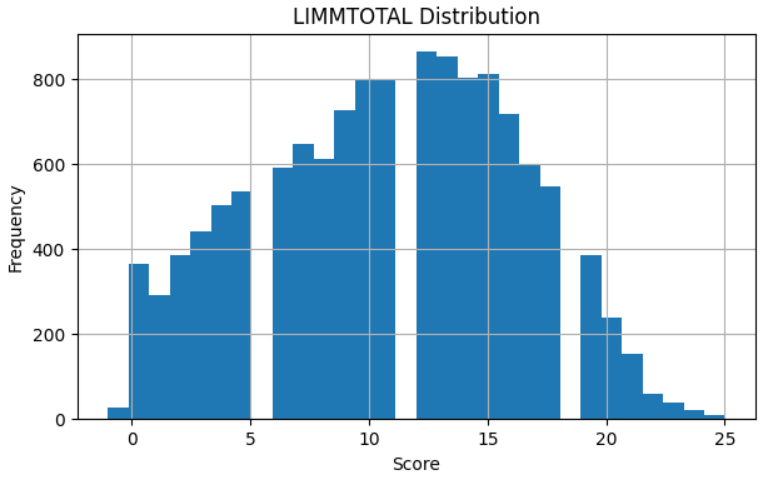
\includegraphics[width=.77\linewidth]{figures/logical_memory_distribution.png}
\caption{Distribution of recorded Logical Memory immediate recall scores (LIMMTOTAL) across visits.}
\label{fig:ritam-logical-memory}
\end{figure}

ADNI records immediate story recall under LIMMTOTAL and delayed recall under LDELTOTAL \cite{adniclinical}. Scores in the histogram cluster most heavily around 10--15, with fewer observations near the upper end of the 0--25 scale. The histogram summarizes visit records, so some participants contribute more than one observation. The modeling pipeline uses one eligible screening or baseline result per participant for each Logical Memory measure.

\clearpage
\subsection{Baseline feature missingness}
The bar chart ranks fields by the percentage of missing values in the baseline data audit. It includes both legacy field names and their baseline-suffixed counterparts, so some measurements appear twice.

\begin{figure}[!ht]
\centering
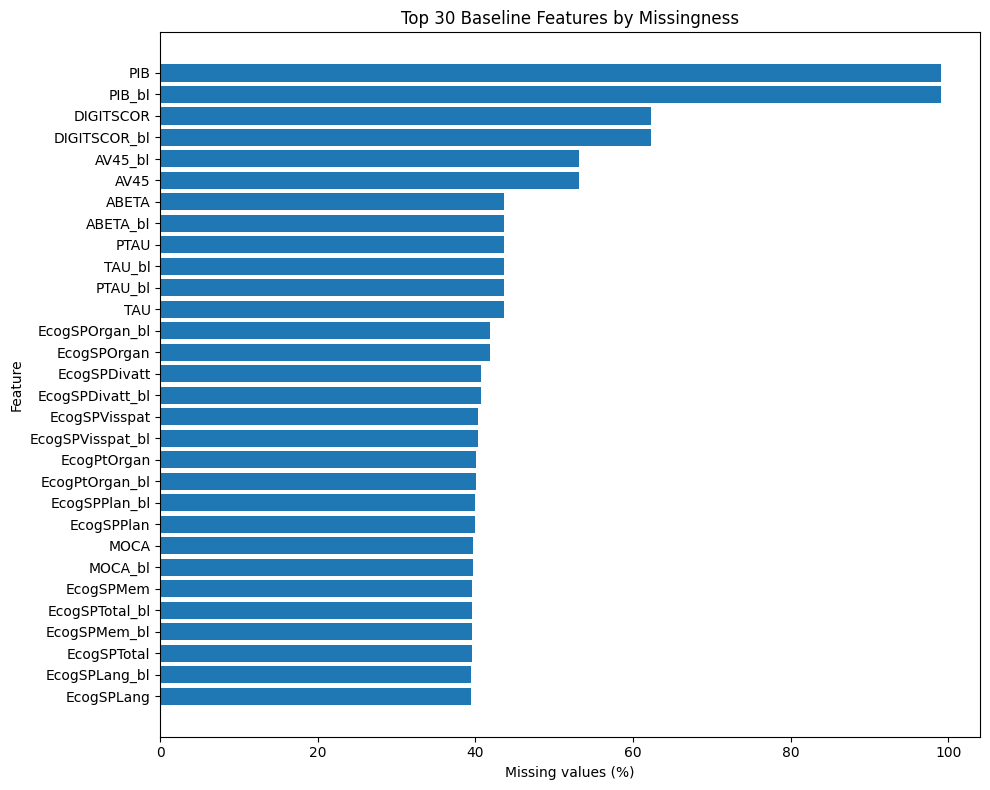
\includegraphics[width=.94\linewidth]{figures/feature_missingness.png}
\caption{Thirty source fields with the highest baseline missingness in the exploratory audit.}
\label{fig:ritam-missingness}
\end{figure}

PIB amyloid PET is missing in about 99\% of records, compared with about 62\% for the digit-symbol score and 53\% for AV45 amyloid PET. The CSF markers ABETA, TAU and PTAU are each missing in roughly 44\%, while several ECog fields and MoCA are around 40--42\%. Similar percentages can suggest shared collection patterns, but participant-level checks are needed to establish whether the same records are missing. The bar chart alone cannot establish the mechanism behind missingness \cite{rubinmissing}. The pipeline used training data to filter features above 80\% missingness and to fit imputation for retained features.
